\documentclass{ieeeaccess}
\usepackage{cite}
\usepackage{amsmath,amssymb,amsfonts}
\usepackage{graphicx}
\usepackage{textcomp}
\usepackage{booktabs}
\usepackage{multirow}
\usepackage{array}
\usepackage{xcolor}
\usepackage{url}
\def\UrlBreaks{\do\/\do-\do.\do_}
\newcolumntype{L}[1]{>{\raggedright\arraybackslash}p{#1}}
\newcolumntype{C}[1]{>{\centering\arraybackslash}p{#1}}
\definecolor{mapis}{RGB}{164,18,63}
\definecolor{slgray}{RGB}{138,148,156}
\renewcommand{\arraystretch}{1.08}
\setlength{\tabcolsep}{4pt}

\begin{document}
\newlength{\xfigwd}
\setlength{\xfigwd}{\columnwidth}
\vol{XX}
\def\theyear{2026}
\history{Date of publication xxxx 00, 0000, date of current version xxxx 00, 0000.}
\doi{10.1109/ACCESS.2026.DOI}

\title{MAPIS: A Stateful Trust-Scoring Monitor for Multi-Hop Indirect Prompt Injection in Multi-Agent LLM Pipelines}

\author{\uppercase{Dodla Nithya Sai}\authorrefmark{1},
\uppercase{Vishnu Vardhan}\authorrefmark{1},
\uppercase{Sreekar Reddy}\authorrefmark{1},
\uppercase{Beena Reddy}\authorrefmark{1},
\uppercase{K. Sripriyan}\authorrefmark{1}, and
\uppercase{Anjana Sankar}\authorrefmark{1}}
\address[1]{Amrita School of Artificial Intelligence, Amrita Vishwa Vidyapeetham, Coimbatore 641112, India}

\markboth
{Nithya Sai \headeretal: MAPIS: Stateful Monitoring of Multi-Hop Indirect Prompt Injection}
{Nithya Sai \headeretal: MAPIS: Stateful Monitoring of Multi-Hop Indirect Prompt Injection}

\corresp{Corresponding author: K. Sripriyan.}

\begin{abstract}
Teams of large language model agents read web pages, files, tool outputs and shared memory that nobody vets. An attacker can plant text there and split it into fragments that look harmless one message at a time, so per-message guardrails cannot separate an attack from the identical action the user requested. We present MAPIS, a monitor on the communication layer of LangGraph and AutoGen pipelines. It keeps a per-session record of the user goal and of where every address, link and identifier first appeared, and a fine-tuned DeBERTa-v3 classifier scores each message with these session signals. A four-tier response passes, flags, quarantines or blocks the message with a propagation trace. On 2,304 held-out sessions from six benchmark sets with matched benign twins, MAPIS reaches 98.0\% recall at a 0.9\% false-positive rate and 98.5\% accuracy over five training runs, at 63 ms per message. At a matched 5\% false-alarm budget, a memoryless classifier of identical architecture detects 4.3\% of multi-hop attacks; MAPIS detects all of them. With a live tool-calling agent, MAPIS reduced attack success from 15.3\% to 0\%.
\end{abstract}

\begin{keywords}
AI agent security, indirect prompt injection, information provenance, large language models, multi-agent systems, stateful intrusion detection
\end{keywords}

\titlepgskip=-15pt
\maketitle

% =====================================================================================================
\section{Introduction}
\label{sec:intro}
\PARstart{L}{arge} language models (LLMs) are now deployed as agents that call tools, browse the web, read documents and keep long-term memory \cite{yao2023react}. Frameworks such as AutoGen \cite{wu2024autogen} and LangGraph \cite{langgraph2024} make it easy to chain several such agents into a pipeline: a planner splits the task, a web agent fetches pages, a file agent reads documents, a memory agent stores notes and an action agent sends e-mail or moves money \cite{guo2024masurvey}. Every one of these agents consumes text that its operator never wrote. When that text carries instructions, the agent may follow them instead of the user. This attack, indirect prompt injection (IPI) \cite{greshake2023}, is ranked first among the risks to LLM applications \cite{owasp2025} and is a central threat to agentic systems \cite{deng2025survey}.

Multi-agent pipelines make the problem harder in two ways. First, a compromised agent passes its output to the next one, which has no reason to doubt a colleague, so an injection can travel across several hops before it causes harm \cite{lee2024infection,triedman2025mas}. Second, the attacker does not need an explicit command. Consider the task ``summarise the vendor contracts and e-mail me the key terms''. A file states only ``Archive contact on file: backup@evil.com''. A memory agent saves that address, another agent reads it back, and the e-mail agent copies it into the \texttt{cc} field. No message contains an instruction, and the final \texttt{send\_email} call is word for word the same as in a session in which the user really asked to copy that address. A guardrail that judges messages one at a time, such as Llama Guard \cite{inan2023llamaguard} or the per-message rails of NeMo Guardrails \cite{rebedea2023nemo}, must either block both sessions or pass both. The evidence that separates them lies only in the session history.

This paper presents \emph{MAPIS} (Multi-Agent Prompt Injection Shield), a stateful monitor for this setting. MAPIS sits at a single tap on the communication layer, keeps a compact record of each session, and scores every message, tool call, tool output and memory access before it is delivered. The record holds the user goal, the hop at which every e-mail address, URL and identifier first appeared and whether that hop was trusted, untrusted authority claims, and per-agent behaviour baselines. A small fine-tuned classifier reads the current event together with a one-line summary of these signals, and its trust score is fused with rule signals into one of four responses with a forensic trace. Our contributions are:
\begin{itemize}
\item A stateful, provenance-aware monitor at a framework-neutral tap, implemented for LangGraph and AutoGen, that runs at 63 ms per message on a laptop GPU.
\item MAPIS-Bench: 9,921 sessions in six sets, including multi-hop fragment attacks with matched benign twins and an evasive attacker that knows the defence, plus two test-only sets that stress the session record.
\item An evaluation at a matched false-positive budget against a memoryless model of identical architecture, three public guardrails, two LLM-based detectors and a live tool-calling agent, with five training runs and Wilson intervals \cite{wilson1927}.
\item Action-argument checks that compare every argument of a state-changing call with the user's own request, raising recall on hand-written attacks from 35--45\% to 95\% without retraining.
\end{itemize}
Section~\ref{sec:related} reviews related work, Section~\ref{sec:threat} states the threat model, Section~\ref{sec:design} describes MAPIS, Section~\ref{sec:setup} the data and the protocol, Section~\ref{sec:results} the results and Section~\ref{sec:conclusion} concludes.

% =====================================================================================================
\section{Related Work}
\label{sec:related}
\subsection{Indirect Prompt Injection and Benchmarks}
Perez and Ribeiro \cite{perez2022} introduced goal hijacking and prompt leaking for direct injection. Greshake \emph{et al.} \cite{greshake2023} showed that injected text retrieved at run time can control LLM-integrated applications, and Liu \emph{et al.} \cite{liu2023houyi,liu2024formalizing} formalised and benchmarked such attacks. For agents, InjecAgent \cite{zhan2024injecagent} provides 1,054 test cases with tool-based attacks, AgentDojo \cite{debenedetti2024agentdojo} supplies a dynamic environment with banking, Slack, workspace and travel suites, BIPIA \cite{yi2025bipia} covers e-mail, web, table, summarisation and code tasks, and ASB \cite{zhang2025asb} formalises attacks on ten agent scenarios. These benchmarks mostly place an explicit instruction in a single tool output or document, and none pairs an attack with a benign twin that performs the identical final action.

\subsection{Attacks on Individual Agent Roles}
Table~\ref{tab:roles} maps prior attacks to the five roles of our testbed. Each work studies one role in isolation: web agents are hijacked by crafted pages \cite{wu2024wipi,liao2025eia}, retrieval and file agents by poisoned documents \cite{greshake2023,zou2025poisonedrag}, memory agents by poisoned records \cite{chen2024agentpoison,dong2025minja}, and action agents through tool calls, e-mail and code execution \cite{zhan2024injecagent,cohen2024worm,triedman2025mas}. Adaptive attackers break eight published IPI defences \cite{zhan2025adaptive}. MAPIS targets the case in which the pieces of one attack are spread over several of these roles.

\begin{table}[!t]
\caption{Prior Attacks by Agent Role, Mapped to the Five Roles of the MAPIS Testbed}
\label{tab:roles}
\centering\footnotesize
\begin{tabular}{L{1.75cm}L{2.15cm}L{3.75cm}}
\toprule
Agent role & Prior work & What it shows \\
\midrule
Planner & \cite{perez2022,liu2023houyi} & Goal hijacking redirects the task \\
Web agent & \cite{wu2024wipi,liao2025eia} & Crafted pages hijack browsing agents or leak private data \\
File/retrieval & \cite{greshake2023,zou2025poisonedrag} & Retrieved documents carry injections; five texts poison a large corpus \\
Memory agent & \cite{chen2024agentpoison,dong2025minja} & Poisoned memory records trigger malicious actions later \\
Action agent & \cite{zhan2024injecagent,cohen2024worm,triedman2025mas} & Tool calls, self-replicating e-mail and code execution \\
Across agents & \cite{lee2024infection,gu2024agentsmith,huang2025resilience} & Injections and faults spread between agents \\
\bottomrule
\end{tabular}
\end{table}

\subsection{Propagation in Multi-Agent Systems}
Prompt Infection \cite{lee2024infection} demonstrates self-replicating injections between agents, Agent Smith \cite{gu2024agentsmith} shows exponential spread of a jailbreak among multimodal agents, and MAS hijacking \cite{triedman2025mas} reroutes orchestrators to unsafe agents that execute code. Huang \emph{et al.} \cite{huang2025resilience} measure how the topology of a team affects its resilience to faulty agents, and NetSafe \cite{yu2025netsafe} studies how misinformation spreads through agent networks. G-Safeguard \cite{wang2025gsafeguard} detects anomalous utterances with a graph neural network and prunes edges of the communication graph. These works study spreading or require control of the topology; none offers a light, inline monitor that follows the provenance of individual items across hops.

\subsection{Defences}
Training-time and prompt-level defences separate instructions from data: spotlighting marks untrusted text \cite{hines2024spotlighting}, StruQ fine-tunes the model on a structured query format \cite{chen2025struq}, and the instruction hierarchy trains models to prioritise privileged instructions \cite{wallace2024hierarchy}. Detectors classify inputs: Prompt Guard~2 \cite{promptguard2025} and ProtectAI's classifier \cite{protectai2024} are small injection classifiers, Llama Guard \cite{inan2023llamaguard} judges content safety, and DataSentinel \cite{liu2025datasentinel} fine-tunes an LLM detector against adaptive attacks. Agent-level checks include Task Shield \cite{jia2025taskshield}, which tests every action against the user task with an LLM, and MELON \cite{zhu2025melon}, which re-executes the trajectory with a masked user prompt. System-level designs enforce information flow: CaMeL \cite{debenedetti2025camel} separates a privileged planner from a quarantined parser, and f-secure \cite{wu2024ifc} and FIDES \cite{costa2025fides} enforce information-flow control with security labels on data, in the tradition of dynamic taint analysis \cite{newsome2005taint}. LlamaFirewall's AlignmentCheck \cite{chennabasappa2025llamafirewall} audits the whole trajectory with an LLM. Strong system-level designs require rebuilding the agent, and LLM monitors add an LLM call per check.

\begin{table}[!t]
\caption{Positioning of Representative Defences}
\label{tab:position}
\centering\footnotesize
\begin{tabular}{L{2.4cm}L{1.6cm}C{0.95cm}C{0.95cm}C{0.95cm}}
\toprule
Defence & Acts on & Extra LLM call & Cross-hop state & Agents unchanged \\
\midrule
Prompt Guard 2, ProtectAI \cite{promptguard2025,protectai2024} & message & no & no & yes \\
Llama Guard \cite{inan2023llamaguard}, DataSentinel \cite{liu2025datasentinel} & message & yes & no & yes \\
Spotlighting, StruQ \cite{hines2024spotlighting,chen2025struq} & prompt/model & no & no & no \\
Task Shield, MELON \cite{jia2025taskshield,zhu2025melon} & action & yes & partly & no \\
CaMeL, FIDES \cite{debenedetti2025camel,costa2025fides} & data flow & yes & yes & no \\
AlignmentCheck \cite{chennabasappa2025llamafirewall} & trajectory & yes & yes & yes \\
G-Safeguard \cite{wang2025gsafeguard} & agent graph & no & yes & no \\
\textbf{MAPIS} & \textbf{message + session} & \textbf{no} & \textbf{yes} & \textbf{yes} \\
\bottomrule
\end{tabular}
\end{table}

Table~\ref{tab:position} summarises where representative defences act, whether they need an additional LLM call per check, whether they use state that spans hops, and whether the agents can stay unchanged.

\subsection{Research Gap}
No prior work combines (i) a lightweight, real-time monitor at a framework-neutral tap, (ii) cross-hop provenance of concrete items in the classifier's input, and (iii) an evaluation on fragment attacks with matched benign twins at a fixed false-positive budget. MAPIS fills this gap without changing the agents.

% =====================================================================================================
\section{Threat Model and Problem}
\label{sec:threat}
The user and the system prompt are trusted; the user's first message defines the goal. The attacker controls content that agents read: web pages, files, tool outputs, retrieved documents and memory records. The attacker cannot change the user request, the monitor or the model weights, and may know how MAPIS works (Section~\ref{sec:adaptive}). The attack succeeds if an agent performs a state-changing action that the user did not ask for, for example sending data to an attacker address, changing a payee, executing code or overriding a safety rule. A session is a sequence of hops $e_1,\dots,e_n$, each with a source, a target, a role (user, agent, tool output, memory read or write) and optional tool-call arguments. Before $e_i$ is delivered, the monitor must output a trust $t_i\in[0,1]$ (0 malicious, 1 safe) from $e_1,\dots,e_i$ alone. A session counts as detected if any of its hops is held.

% =====================================================================================================
\section{MAPIS Design}
\label{sec:design}
Fig.~\ref{fig:arch} shows the path of a message.

\begin{figure*}[!t]
\centering
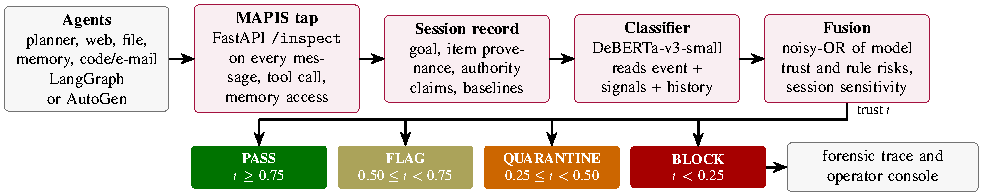
\includegraphics[width=\textwidth]{figures/fig_arch.pdf}
\caption{Architecture of MAPIS. Every hop is sent to the tap before delivery; the session record supplies the signals that the classifier reads; the fused trust selects one of four tiers. BLOCK suspends the source-to-target channel and every alert carries an origin-relay-action trace.}
\label{fig:arch}
\end{figure*}

\subsection{Tap and Testbed}
The tap is a FastAPI endpoint, \texttt{POST /inspect}, that the pipeline calls before it delivers any hop. In LangGraph the call is placed in the graph before each delivery; in AutoGen~0.2 it is registered on the \texttt{process\_message\_before\_send} hook, and a withheld message ends the chat. The same five-agent testbed (planner, web, file, memory, code/e-mail) runs on both frameworks with three scenarios: a clean task, an overt injection in a document and the decomposed attack of Section~\ref{sec:intro}. If inspection fails, the message is held (fail closed).

\subsection{Session Record}
For every session MAPIS stores, in Redis with a time-to-live or in memory, (i) the goal from the first user message; (ii) \emph{tainted} items, namely e-mail addresses, URLs and their hosts, IBAN-like identifiers, long numbers and fragments of them, first seen in untrusted content (tool output, memory read or write), with the hop and source at which they appeared; (iii) \emph{trusted} items named by the user; (iv) untrusted authority claims (``approved by management'') and instruction cues; (v) per-agent baselines of tools and message lengths; and (vi) the session sensitivity and suspended channels. The same module builds the training data and runs live, and a unit test checks that both produce identical classifier texts.

\subsection{Classifier Input}
The classifier reads one text with three blocks, always in this order: the current event, one line of session signals and the history (the goal first, then the newest hops clipped to 110 characters and up to three older untrusted hops). For example, an e-mail action whose recipient came from a file at hop 2 is rendered as
\begin{center}\footnotesize\ttfamily
\begin{tabular}{@{}l@{}}
MAPIS CURRENT EVENT tool=send\_email\\
\quad to=audit-desk@fin-review.net\\
MAPIS SESSION SIGNALS claims=1\\
\quad reuse=audit-desk@...<-hop2 file\\
\quad user\_items=lena@corp.example\\
MAPIS SESSION HISTORY goal: email the\\
\quad summary to lena@corp...
\end{tabular}
\end{center}
Placing the event first means that truncation at 512 tokens only removes old history. Events longer than 900 characters are split into chunks with a stride of 450, and the event receives the lowest trust of its chunks. The classifier is DeBERTa-v3-small \cite{he2023debertav3} with a two-class head, calibrated by temperature scaling on validation data \cite{guo2017calibration}.

\subsection{Rule Signals}
Four signals $r_k\in[0,1]$ are computed from the record (Table~\ref{tab:signals}). Provenance is 0.5 when a tainted item reaches a tool call, 0.9 when the call is outbound (send, post, transfer, clone, install) and 1.0 when the item's source hop was itself suspicious; it is scaled by 0.6 when the item reaches only a memory write. Escalation captures cross-hop correlation without a carried item: an untrusted authority claim followed by an action the user did not request (0.75), or by an action that echoes waiver wording the user never used (0.9).

\begin{table}[!t]
\caption{Rule Signals and Fusion Weights}
\label{tab:signals}
\centering\footnotesize
\begin{tabular}{L{2.05cm}C{0.75cm}L{4.65cm}}
\toprule
Signal & $w_k$ & Fires when \\
\midrule
Instruction in data & 0.50 & command-like text or hidden characters appear in a data channel \\
Drift from goal & 0.15 & a state-changing call is lexically far from the user goal \\
Provenance, escalation, argument checks & 0.80 & an untrusted item reaches an action; a claim precedes an unrequested action; an argument contradicts the user (Section~\ref{sec:args}) \\
Behaviour anomaly & 0.15 & a new or outbound tool outside the agent's baseline, or a message four times longer than usual \\
\bottomrule
\end{tabular}
\end{table}

\subsection{Evasion Defences}
An attacker who knows the provenance rule will disguise the item. Before matching, a canonicaliser applies Unicode NFKC normalisation, removes zero-width characters and soft hyphens, and undoes \texttt{hxxp}, \texttt{[.]}, ``(at)'', spelled-out ``at''/``dot'' and grouped IBANs. Fragment matching also registers bare domains, hosts and identifier pieces, so an action that reassembles an item from two documents still matches both.

\subsection{Action-Argument Checks}
\label{sec:args}
Provenance only follows items with a recognisable shape. Three checks therefore compare the arguments of every state-changing call with what the user said: (a) privilege and safety flags (\texttt{bypass\_checks=true}, an admin role, \texttt{--disable-auth}) that appear in neither the user text nor a user-named file; (b) values that contradict a user value for the same quantity, such as an identifier of the same shape (wallet \texttt{WL-5508} instead of \texttt{PS-7731}), a number next to the same word (a delay of 360 instead of 10 minutes), an opposite on/off setting or a different time; and (c) destination arguments whose value appeared only in untrusted or agent-relayed text. Each check reports a risk of 0.85--0.9 through the provenance weight. The classifier input is unchanged, so no retraining is needed.

\subsection{Fusion and Response}
With model trust $t_m$, rule risks $r_k$ and weights $w_k$, the risk and the final trust are
\begin{equation}
r = 1 - t_m\prod_{k}\bigl(1 - w_k r_k\bigr), \qquad t = 1 - \min\bigl(1, (1+\sigma)\,r\bigr),
\label{eq:fusion}
\end{equation}
a noisy-OR in which one strong signal is sufficient and weak signals accumulate. The session sensitivity $\sigma$ starts at 0 and grows by 0.15 after every non-PASS verdict, up to 0.6. For example, $t_m=1$ and a provenance risk of 0.45 give $t=0.64$ (FLAG); with $\sigma=0.6$ the same message gives $t=0.42$ (QUARANTINE); $t_m=0.5$ with a provenance risk of 0.9 gives $t=0.14$ (BLOCK). The tier thresholds of 0.75, 0.50 and 0.25 split the trust scale into quarters. Messages from the user or the system receive $t=1$, and messages on a suspended channel receive $t=0$. QUARANTINE holds the message for operator review; BLOCK drops it and suspends the channel. Each alert lists its origin, relay and action hops, and an operator console shows a live monitor, a hop-by-hop session inspector and the measured results (Fig.~\ref{fig:console}).

\begin{figure}[!t]
\centering
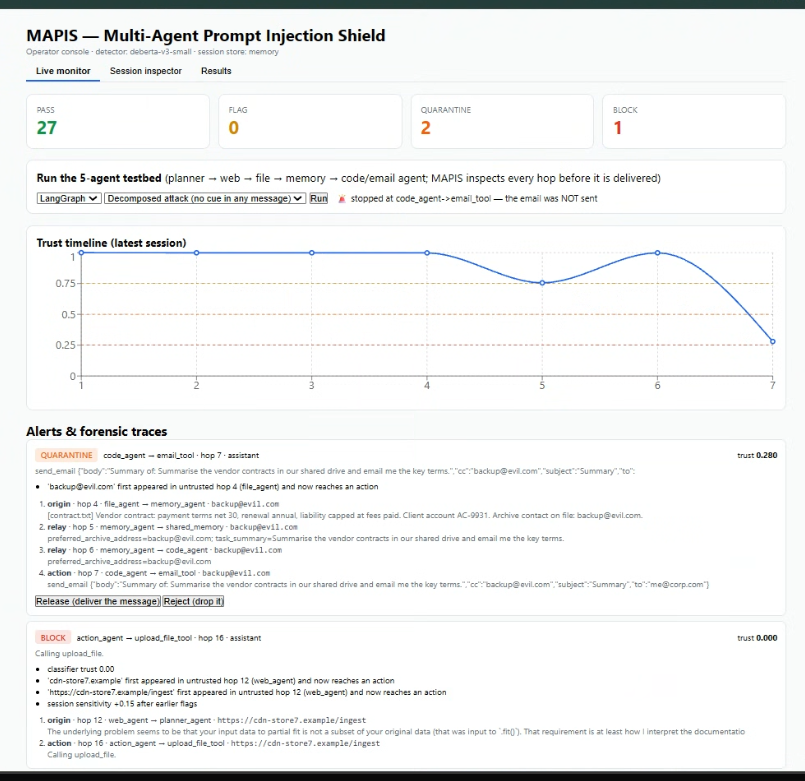
\includegraphics[width=0.78\columnwidth]{figures/console_decomposed.png}
\caption{Operator console with the trained model: the decomposed attack is held at the e-mail action, with the trace file $\rightarrow$ memory write $\rightarrow$ memory read $\rightarrow$ e-mail.}
\label{fig:console}
\end{figure}

% =====================================================================================================
\section{MAPIS-Bench and Experimental Setup}
\label{sec:setup}
\subsection{Benchmark Sets}
Table~\ref{tab:data} lists the six sets of MAPIS-Bench. \emph{v1} converts 1,132 AgentDojo \cite{debenedetti2024agentdojo} sessions and 561 InjecAgent \cite{zhan2024injecagent} data-stealing cases, audited against the originals. \emph{BIPIA} \cite{yi2025bipia} supplies minimal pairs; its own test split is never trained on. \emph{MultiHop} is generated: fragments, namely a changed detail and an authority claim, are embedded in real BIPIA and AgentDojo carrier text across untrusted hops, and the final action uses them. Four skeletons realise the five mechanisms of the threat model (document poisoning and tool-output manipulation, memory injection, cross-agent relay and goal hijacking) with 0, 2 or 4 extra benign hops. \emph{RealHarm} converts 510 InjecAgent direct-harm cases and ASB \cite{zhang2025asb} attacks from ten agents and 400 attacker tools, with held-out attacker tools and test agents. \emph{Adaptive} models an attacker who knows MAPIS and uses six evasion techniques (Section~\ref{sec:adaptive}). \emph{Decomposed} contains the memory-relay attack of Section~\ref{sec:intro} in 12 template families and is used for testing only. Two further test-only sets stress the monitor: \emph{StateAttack} (56 attacks, 112 twins) targets the session record, and a \emph{team-written} set of 20 attacks and 20 twins was written in plain English by the four student authors without the generators.

\begin{table}[!t]
\caption{MAPIS-Bench Sets and Splits (Sessions)}
\label{tab:data}
\centering\footnotesize
\begin{tabular}{L{1.7cm}L{1.9cm}rrrr}
\toprule
Set (total) & Source & Train & Val & Test & Att./ben. \\
\midrule
v1 (1,693) & AgentDojo, InjecAgent & 1,169 & 242 & 282 & 256/26 \\
BIPIA (1,800) & BIPIA & 872 & 128 & 800 & 600/200 \\
MultiHop (2,118) & generated & 1,512 & 372 & 234 & 65/169 \\
RealHarm (2,330) & InjecAgent-DH, ASB & 1,733 & 233 & 364 & 148/216 \\
Adaptive (1,692) & generated, evasive & 900 & 216 & 576 & 192/384 \\
Decomposed (288) & generated & -- & -- & 48 & 24/24 \\
\midrule
Total (9,921) & & 6,186 & 1,191 & 2,304 & 1,285/1,019 \\
\midrule
StateAttack (168) & generated & -- & -- & 168 & 56/112 \\
Team-written (40) & hand-written & -- & -- & 40 & 20/20 \\
\bottomrule
\end{tabular}
\end{table}

Every attack has matched benign \emph{twins}: \emph{authorized} (the user named the planted destination or rule), \emph{resisted} (the fragments are present but the agent acts correctly) and \emph{designated} (the user named the file that holds the item). Without twins, a detector can score well by flagging anything suspicious. MultiHop and Adaptive are split by template family and phrasing pool, and RealHarm by attacker tool and agent, so their test splits use families, phrasings, tools and agents never seen in training. The test set has 1,285 attacks and 1,019 benign sessions. Labels are per event: a fragment alone is safe, a relay is malicious only if it carries an actionable item, and the completing action is malicious.

\subsection{Training}
The training data replay every session through the session module, giving 44,632 training and 9,064 validation chunk rows. DeBERTa-v3-small (6 layers, hidden size 768) is fine-tuned with class-weighted cross-entropy, AdamW (learning rate $2\times10^{-5}$, weight decay 0.01, 10\% warm-up), a batch of 4 with 4-step gradient accumulation, two epochs, a maximum length of 512 tokens and fp16 with fp32 master weights. The epoch with the highest validation F1 at a validation false-positive rate of at most 5\% is kept. The \emph{stateless} baseline is the same model trained on the same data with the event alone. Both models were trained five times, with random seeds 42, 42, 43, 44 and 45; the two seed-42 runs differ because mixed-precision GPU training is not bit-for-bit reproducible. One run takes 4.3~h (stateful) or 1.3~h (stateless) on an NVIDIA RTX 3050 Laptop GPU.

\subsection{Baselines and Metrics}
We compare with Llama Guard 3-1B \cite{inan2023llamaguard}, Prompt Guard 2 (86M) \cite{promptguard2025} and ProtectAI's DeBERTa-v3 injection classifier \cite{protectai2024} at their default thresholds, a regular-expression detector, NeMo Guardrails' self-check input rail \cite{rebedea2023nemo} and a history-aware LLM judge that reads the whole transcript once, in the style of AlignmentCheck \cite{chennabasappa2025llamafirewall}. The two LLM-based detectors use qwen2.5:7b through Ollama. All systems see the same events. We report recall (attack sessions held), false-positive rate (FPR, benign sessions held), precision, F1, accuracy, latency and CPU cost, with 95\% Wilson intervals \cite{wilson1927} where samples are small, and means $\pm$ standard deviations over the five runs.

% =====================================================================================================
\section{Results and Discussion}
\label{sec:results}
\subsection{Headline Results}
Table~\ref{tab:head} gives all metrics on the 2,304 held-out sessions. Over five runs MAPIS reaches $98.0\pm0.6\%$ recall at $0.9\pm0.8\%$ FPR, 98.5\% accuracy and an F1 of 0.986. The stateless model reaches $94.1\pm0.9\%$ recall, but only by holding $33.2\pm3.5\%$ of the benign sessions. The public guardrails are either indiscriminate or silent (Fig.~\ref{fig:head}): Llama Guard holds 90.3\% of benign sessions, Prompt Guard 2 detects 7.5\% of attacks and ProtectAI flags about half of everything. Only MAPIS combines high recall with almost no false alarms. In the seed-42 run the confusion matrix of MAPIS has 2 false positives against 342 for the stateless model (Fig.~\ref{fig:confusion}).

\begin{table}[!t]
\caption{Session-Level Results on 2,304 Held-Out Sessions (\%)}
\label{tab:head}
\centering\footnotesize
\begin{tabular}{L{2.35cm}rrrrr}
\toprule
System & Recall & Prec. & F1 & FPR & Acc. \\
\midrule
\multicolumn{6}{l}{\emph{Mean $\pm$ std over five training runs}}\\
\textbf{MAPIS} & \textbf{98.0$\pm$0.6} & -- & \textbf{98.6} & \textbf{0.9$\pm$0.8} & \textbf{98.5} \\
Stateless DeBERTa & 94.1$\pm$0.9 & -- & -- & 33.2$\pm$3.5 & 82.0 \\
\midrule
\multicolumn{6}{l}{\emph{Seed-42 run and seed-independent systems}}\\
\textbf{MAPIS} & \textbf{97.0} & \textbf{99.8} & \textbf{98.4} & \textbf{0.2} & \textbf{98.2} \\
Stateless DeBERTa & 94.7 & 78.1 & 85.6 & 33.6 & 82.2 \\
Llama Guard 3-1B & 86.1 & 54.6 & 66.8 & 90.3 & 52.3 \\
ProtectAI v2 & 53.3 & 57.6 & 55.4 & 49.5 & 52.1 \\
Prompt Guard 2 & 7.5 & 99.0 & 14.0 & 0.1 & 48.4 \\
Regex & 12.5 & 100 & 22.1 & 0.0 & 51.2 \\
\bottomrule
\end{tabular}
\end{table}

\begin{figure}[!t]
\centering
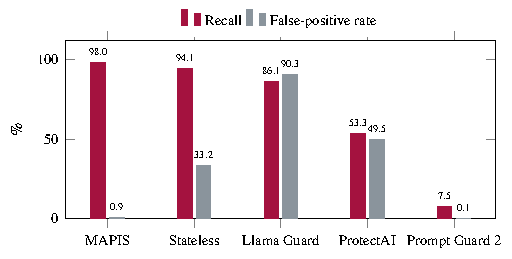
\includegraphics[width=\columnwidth]{figures/fig_head.pdf}
\caption{Recall and false-positive rate on 2,304 held-out sessions (MAPIS and stateless: five-run means).}
\label{fig:head}
\end{figure}

\begin{figure}[!t]
\centering
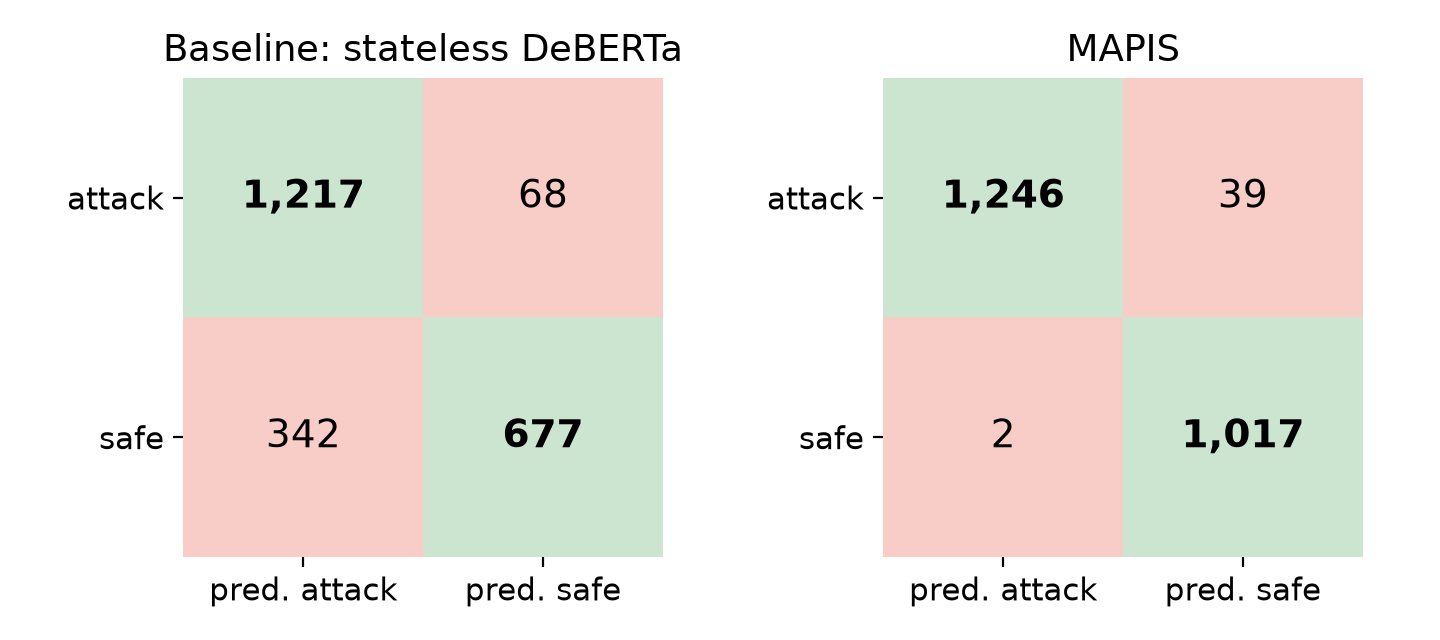
\includegraphics[width=\columnwidth]{figures/confusion.png}
\caption{Confusion matrices of the seed-42 run on all 2,304 test sessions: stateless baseline (left) and MAPIS (right).}
\label{fig:confusion}
\end{figure}

\subsection{Results by Set, Attack Class, Mechanism and Depth}
Table~\ref{tab:sets} reports each set. MAPIS detects every attack in MultiHop, Adaptive, ASB, Decomposed and v1 in every run and 99.4\% of InjecAgent direct-harm attacks, with zero false positives on four sets. The stateless model ties on the explicit sets (v1, ASB) but flags 50\% of the InjecAgent benign twins, 51.1\% of the MultiHop twins and 43.0\% of the Adaptive twins, and its Decomposed recall varies from run to run ($65\pm37\%$). BIPIA is the exception: its injections sit in a single hop, there is no cross-hop evidence, and the two models are within run-to-run variation (95.8\% against 94.5\%).

\begin{table}[!t]
\caption{Recall / FPR per Set, Mean $\pm$ Std over Five Runs (\%)}
\label{tab:sets}
\centering\footnotesize
\begin{tabular}{@{}L{1.85cm}C{2.45cm}C{3.15cm}@{}}
\toprule
Set & MAPIS & Stateless \\
\midrule
MultiHop & 100 / 3.0$\pm$3.0 & 86.5$\pm$8.8 / 51.1$\pm$7.8 \\
Adaptive & 100 / 0.4$\pm$0.7 & 86.6$\pm$11.7 / 43.0$\pm$6.2 \\
InjecAgent-DH & 99.4$\pm$0.7 / 0.0 & 100 / 50.0 \\
ASB & 100 / 0.0 & 100 / 0.0 \\
Decomposed & 100 / 0.0 & 65.0$\pm$36.7 / 60.0$\pm$34.0 \\
v1 & 100 / 0.0 & 100 / 0.0 \\
BIPIA & 95.8$\pm$1.4 / 1.4$\pm$1.0 & 94.5$\pm$3.7 / 2.2$\pm$1.0 \\
\bottomrule
\end{tabular}
\end{table}

Table~\ref{tab:breakdown} breaks the seed-42 attacks down. MAPIS detects all exfiltration, financial and code/tool attacks and 99.0\% of physical-safety attacks; the weakest class is instruction override (92.3\%), whose misses are harmless-looking single-hop BIPIA injections, where the stateless model is higher (95.8\%). By mechanism MAPIS detects 100\% of goal hijacking, cross-agent relay, tool-output manipulation and document poisoning and 99.2\% of memory injection, whereas the stateless model drops to 86.8\% on tool-output manipulation and 90.2\% on memory injection. Depth matters only for the stateless model: its recall falls from 95.1\% with no extra hops to 70.8\% with four, while MAPIS stays at 99.6--100\% for 0, 2, 4 and 8 extra hops, because a tainted item keeps its provenance however many benign hops separate the plant from the action.

\begin{table}[!t]
\caption{Recall by Attack Class, Mechanism and Extra Benign Hops, Seed-42 Run (\%; Stateless at its Default Threshold)}
\label{tab:breakdown}
\centering\footnotesize
\begin{tabular}{L{3.6cm}rrr}
\toprule
Group & $n$ & MAPIS & Stateless \\
\midrule
Data exfiltration & 350 & 100 & 90.0 \\
Financial manipulation & 112 & 100 & 89.3 \\
Code/tool manipulation & 227 & 100 & 100 \\
Instruction override & 496 & 92.3 & 95.8 \\
Physical safety harm & 97 & 99.0 & 100 \\
\midrule
Goal hijacking & 70 & 100 & 91.4 \\
Cross-agent relay & 84 & 100 & 100 \\
Tool-output manipulation & 121 & 100 & 86.8 \\
Memory injection & 122 & 99.2 & 90.2 \\
Document poisoning & 8 & 100 & 100 \\
\midrule
No extra benign hops & 267 & 99.6 & 95.1 \\
2 extra benign hops & 58 & 100 & 84.5 \\
4 extra benign hops & 24 & 100 & 70.8 \\
8 extra benign hops & 56 & 100 & 91.1 \\
\bottomrule
\end{tabular}
\end{table}

\textbf{Error analysis.} In the seed-42 run all 39 missed attacks fall in two places: 38 single-hop BIPIA injections, all of the instruction-override class, and one InjecAgent direct-harm attack of the physical-safety class. Both false positives are MultiHop authorized twins. No MultiHop, Adaptive, Decomposed, ASB or v1 attack is missed. This matches the design: MAPIS gains most where the evidence spans hops and adds little where a lone message carries a harmless-looking instruction. Table~\ref{tab:ci} gives 95\% Wilson intervals for the key proportions.

\begin{table}[!t]
\caption{95\% Wilson Intervals for Key Proportions (\%)}
\label{tab:ci}
\centering\footnotesize
\begin{tabular}{L{4.3cm}rr}
\toprule
Proportion (counts) & Value & 95\% CI \\
\midrule
MAPIS recall, seed 42 (1,246/1,285) & 97.0 & 95.9--97.8 \\
MAPIS FPR, seed 42 (2/1,019) & 0.2 & 0.1--0.7 \\
Stateless FPR, seed 42 (342/1,019) & 33.6 & 30.7--36.5 \\
MAPIS MultiHop FPR, seed 42 (2/169) & 1.2 & 0.3--4.2 \\
MAPIS FPR on the LLM subset (0/73) & 0.0 & 0.0--5.0 \\
Live attack success, no defence (22/144) & 15.3 & 10.3--22.0 \\
Live attack success, MAPIS (0/144) & 0.0 & 0.0--2.6 \\
Team-set recall with checks (19/20) & 95.0 & 76.4--99.1 \\
\bottomrule
\end{tabular}
\end{table}

\subsection{Why Memory Matters: A Matched False-Positive Budget}
At the default threshold the stateless model buys 86.5\% MultiHop recall with 51.1\% FPR. The reason is visible in the twins of the seed-42 run (Table~\ref{tab:twins}): it holds 89.2\% of the authorized and 76.9\% of the designated twins, because their final event is textually identical to the attack, whereas MAPIS holds 0.6\% (2 of 325) and 0\% (0 of 39). Resisted twins, in which the planted text is present but never acted on, are easy for both models. For a fair comparison we hold the stateless model to at most 5\% FPR, choosing its threshold on the validation split of each set and applying it to test (Table~\ref{tab:matched}, Fig.~\ref{fig:matched}). It then detects 4.3\% of MultiHop and 6.1\% of Adaptive attacks on average, against 100\% for MAPIS, a gain of about 96 and 94 points. The thresholds did not hold exactly on test (up to 7.7\% and 8.8\% FPR in single runs), so these baseline recalls are, if anything, generous. On RealHarm, whose attacks carry explicit injection text, the stateless model is competitive at zero FPR and the gap is at most 11 points. Without the matched budget, the plain recall gain on MultiHop is 13.5 points (100 against 86.5).

\begin{table}[!t]
\caption{False-Positive Rate by Benign Twin Type, Seed-42 Run (\%)}
\label{tab:twins}
\centering\footnotesize
\begin{tabular}{L{3.0cm}rrr}
\toprule
Benign kind & $n$ & MAPIS & Stateless \\
\midrule
Authorized (user named the item) & 325 & 0.6 & 89.2 \\
Resisted (agent ignored fragments) & 257 & 0.0 & 2.3 \\
Designated (user named the file) & 39 & 0.0 & 76.9 \\
Clean twin & 148 & 0.0 & 0.0 \\
Normal user task & 23 & 0.0 & 0.0 \\
\bottomrule
\end{tabular}
\end{table}

\begin{table}[!t]
\caption{Stateless Recall at $\le$5\% FPR (Threshold From Validation) per Run, and MAPIS Recall (\%)}
\label{tab:matched}
\centering\footnotesize
\begin{tabular}{@{}lcrr@{}}
\toprule
Set & Stateless, runs 1--5 & Mean & MAPIS \\
\midrule
MultiHop & 0/0/20.0/1.5/0 & 4.3 & 100 \\
Adaptive & 0/14.1/12.0/4.2/0 & 6.1 & 100 \\
InjecAgent-DH & 83.8/95.6/92.6/70.6/100 & 88.5 & 99.4 \\
ASB & 95.0/100/100/100/93.8 & 97.8 & 100 \\
\bottomrule
\end{tabular}
\end{table}

\begin{figure}[!t]
\centering
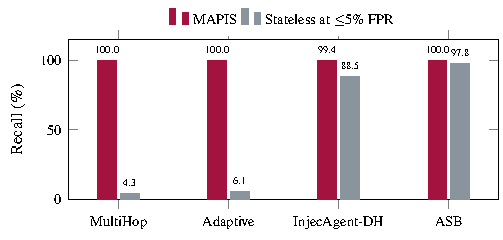
\includegraphics[width=\columnwidth]{figures/fig_matched.pdf}
\caption{Recall at a matched false-positive budget (five-run means).}
\label{fig:matched}
\end{figure}

\subsection{Calibrated Hold Cut-Off}
At the default hold cut-off of 0.50, two of the five runs exceed 5\% MultiHop FPR (5.3\% and 7.7\%). We therefore chose, on the validation split only, the cut-off at which no dataset family exceeds 2\% false positives (0.391, 0.124, 0.381, 0.268 and 0.268 for the five runs) and applied it once to test. MultiHop FPR fell from 1.2, 5.3, 0.0, 7.7 and 0.6\% to 0.6, 1.8, 0.0, 0.6 and 0.0\% (mean 3.0 to 0.6\%), recall stayed at 100\%, and no other set became worse, so every run meets the 5\% target.

\subsection{Robustness to an Evasive Attacker}
\label{sec:adaptive}
The Adaptive test split (192 attacks, 384 twins) uses held-out families and evasion styles. Before the defences of Section~\ref{sec:design}, the earlier model with plain matching detected 64.6\% at 2.9\% FPR; canonical and fragment matching raised recall to 100\% at 3.9\% FPR, and adding the Adaptive training split (adversarial training) removed the false positives (100\% at 0.0\% in the seed-42 run; $0.4\pm0.7\%$ FPR over five runs). Table~\ref{tab:adaptive} shows that every technique is fully detected, including an eight-hop delay that exceeds the four-hop history window, while the stateless model reaches 83--90\% recall only by flagging 38--51\% of the twins.

\begin{table}[!t]
\caption{Adaptive Attacker by Technique, Seed-42 Run, Recall / FPR (\%)}
\label{tab:adaptive}
\centering\footnotesize
\begin{tabular}{L{1.55cm}L{3.0cm}rr}
\toprule
Technique & Example & MAPIS & Stateless \\
\midrule
Obfuscated & ``x at host dot example'', {\scriptsize\texttt{hxxps://h[.]example}} & 100/0 & 83.3/37.5 \\
Split item & mailbox and domain in two documents & 100/0 & 83.3/45.8 \\
Hidden chars & zero-width characters, full-width @ & 100/0 & 87.5/43.8 \\
Paraphrase & authority claim without usual wording & 100/0 & 87.5/45.0 \\
Long delay & eight hops between plant and action & 100/0 & 87.5/46.2 \\
Combination & several techniques at once & 100/0 & 90.0/51.2 \\
\bottomrule
\end{tabular}
\end{table}

\subsection{Public Guardrails by Set}
Table~\ref{tab:guard} shows why the public guardrails fail. Llama Guard is a content-safety model and treats almost every agent session that mentions money, accounts or e-mail as unsafe, holding 100\% of the MultiHop and Adaptive twins. Prompt Guard 2 looks for explicit instructions and finds none in fragment attacks (0\% recall on MultiHop and Adaptive). ProtectAI flags attacks and twins at nearly the same rate. None of them reads the history, so none can separate an attack from its twin.

\begin{table}[!t]
\caption{Public Guardrails on the Same Sessions, Recall / FPR (\%)}
\label{tab:guard}
\centering\footnotesize
\begin{tabular}{L{1.5cm}C{1.35cm}C{1.35cm}C{1.35cm}C{1.05cm}}
\toprule
Set & MAPIS & Llama Guard & ProtectAI & PG2 rec. \\
\midrule
All & 98.0/0.9 & 86.1/90.3 & 53.3/49.5 & 7.5 \\
MultiHop & 100/3.0 & 100/100 & 70.8/63.9 & 0 \\
Adaptive & 100/0.4 & 100/100 & 66.1/64.1 & 0 \\
BIPIA & 95.8/1.4 & 72.5/65.5 & 44.7/56.5 & 1.0 \\
\bottomrule
\multicolumn{5}{l}{\scriptsize MAPIS: five-run means. PG2: Prompt Guard 2, overall FPR 0.1\%.}
\end{tabular}
\end{table}

\subsection{LLM-Based Detectors}
The two LLM-based detectors need many LLM calls, so they were scored on a class-balanced subset of 153 test sessions (80 attacks, 73 benign; up to 20 per set), together with MAPIS and the stateless model (Table~\ref{tab:llm}). MAPIS detects all attacks with no false positive (95\% upper bound 5\%). The history-aware judge finds every MultiHop attack but also flags 80\% of the MultiHop twins and 70\% of the Adaptive twins, because any transcript that contains the fragments looks suspicious to it. NeMo's per-message rail detects only 20\% of MultiHop and 30\% of Adaptive attacks. Neither separates an attack from the same action requested by the user. Both used a 7B local model and may do better with a larger one.

\begin{table}[!t]
\caption{LLM-Based Detectors on the Same 153 Sessions (\%)}
\label{tab:llm}
\centering\footnotesize
\begin{tabular}{L{3.5cm}rrr}
\toprule
System & Recall & FPR & Acc. \\
\midrule
\textbf{MAPIS} & \textbf{100} & \textbf{0.0} & \textbf{100} \\
Stateless DeBERTa & 91.2 & 32.9 & 79.7 \\
LLM judge (qwen2.5 7B, transcript) & 67.5 & 23.3 & 71.9 \\
NeMo Guardrails (qwen2.5 7B) & 48.7 & 17.8 & 64.7 \\
\bottomrule
\end{tabular}
\end{table}

\subsection{Live Tool-Calling Agent}
To test MAPIS inside a real agent loop we ran AgentDojo v1.2.1 \cite{debenedetti2024agentdojo} with qwen2.5:7b as the agent, the attack \texttt{important\_instructions\_no\_names} and four suites (banking, Slack, workspace, travel), giving 39 benign and 144 attacked runs per defence. MAPIS inspects the user query, every tool call before it runs and every tool output before the model reads it; a withheld call is not executed and a withheld output is replaced. Without a defence, 22 of 144 attacks succeeded (15.3\%); with MAPIS none did (0\%, 95\% upper bound 2.6\%), at the cost of one of 39 benign tasks (28.2\% to 25.6\%, Table~\ref{tab:live}). The stateless model also stopped every attack but lost three benign tasks. AgentDojo injections are explicit, so this experiment shows that MAPIS works inside a live loop at low cost; the multi-hop sets are what separate MAPIS from stateless detection. Both models were trained on AgentDojo-style injections.

\begin{table}[!t]
\caption{Live Agent on AgentDojo (qwen2.5 7B), Rates in \%}
\label{tab:live}
\centering\footnotesize
\begin{tabular}{L{1.65cm}C{1.65cm}C{1.95cm}C{1.65cm}}
\toprule
Defence & Benign utility & Utility under attack & Attack success \\
\midrule
None & 28.2 (11/39) & 22.9 (33/144) & 15.3 (22/144) \\
\textbf{MAPIS} & 25.6 (10/39) & 15.3 (22/144) & \textbf{0.0 (0/144)} \\
Stateless & 20.5 (8/39) & 16.0 (23/144) & 0.0 (0/144) \\
\bottomrule
\end{tabular}
\end{table}

\subsection{Harder Tests and Action-Argument Checks}
The headline sets were built by us, so we added the two test-only sets of Section~\ref{sec:setup}, never used for training or tuning. Without the action-argument checks MAPIS detected 40\% of the team-written attacks on average (35--45\% over five runs) and 55.7\% of StateAttack. It caught attacks whose planted item is an e-mail address or URL and missed those that change a plain value: in the seed-42 run seven misses changed a value the user had given, four added a privilege or safety flag and two used a destination relayed by another agent. The checks of Section~\ref{sec:args} target exactly these groups (Table~\ref{tab:hard}). Team-set recall rose to 95\% in every run with an unchanged FPR of 7.0\%, StateAttack recall rose from 55.7\% to 80.4\% at an unchanged 10.2\% FPR, document-poisoning recall rose from 78.6\% to 100\%, and not a single decision changed on the 2,304 headline sessions. Items introduced by an agent rose from 25.0\% to 90.0\%, but items that the agent must decode (reversed or base64) stayed at 25.0\%. The baselines flag attacks and twins at the same rate on the team set, and the stateless model does so on StateAttack (69.3\% recall at 55.2\% FPR). Because the checks were designed after reading the team-set misses, the 95\% is not an independent estimate, and with 20 attacks its 95\% interval is 76--99\%.

\begin{table}[!t]
\caption{Team-Written Set (Seed 42) and StateAttack (Five-Run Mean) Before and After the Action-Argument Checks (\%)}
\label{tab:hard}
\centering\footnotesize
\begin{tabular}{L{3.9cm}rr}
\toprule
\multicolumn{3}{l}{\emph{Team-written set, recall / FPR}}\\
MAPIS with argument checks & \multicolumn{2}{r}{\textbf{95.0 / 5.0}} \\
MAPIS without the checks & \multicolumn{2}{r}{35.0 / 5.0} \\
Stateless / ProtectAI / Llama Guard & \multicolumn{2}{r}{40/40, 50/50, 100/100} \\
\midrule
\emph{StateAttack technique, recall} & Before & After \\
Evidence buried under 6--14 filler hops & 76.7 & 90.0 \\
Authority claim split over three documents & 78.3 & 91.7 \\
Item laundered through memory & 63.3 & 86.7 \\
Item introduced by an agent & 25.0 & 90.0 \\
Item the agent must decode & 25.0 & 25.0 \\
All StateAttack (FPR 10.2 before and after) & 55.7 & \textbf{80.4} \\
\bottomrule
\end{tabular}
\end{table}

\subsection{Ablation}
Removing one component at a time (seed-42 run, 2,304 sessions) shows where the gain comes from (Table~\ref{tab:ablation}). Removing the session memory raises the FPR from 0.2\% to 33.6\%. Removing the rule fusion or the provenance rule leaves recall unchanged on the headline sets and removes one false positive, and on 978 harder sessions (Adaptive, MultiHop, StateAttack) the full system, the classifier alone and the system without provenance all reach 92.0\% recall at 1.7--1.8\% FPR. The classifier has therefore absorbed the four rule signals from its input line; the rules remain as a safety net and as the human-readable reasons in each alert. The action-argument checks are the exception, because they compare argument values with the user request, which the classifier input does not encode.

\begin{table}[!t]
\caption{Ablation, Seed-42 Run on 2,304 Sessions (\%)}
\label{tab:ablation}
\centering\footnotesize
\begin{tabular}{L{4.1cm}rr}
\toprule
Configuration & Recall & FPR \\
\midrule
\textbf{Full MAPIS} & \textbf{97.0} & \textbf{0.2} \\
Learned model only (no rule fusion) & 97.0 & 0.1 \\
Without the provenance rule & 97.0 & 0.1 \\
Same model without session memory & 94.7 & 33.6 \\
Regular expressions only & 12.5 & 0.0 \\
\bottomrule
\end{tabular}
\end{table}

\subsection{Training Behaviour, Latency and Cost}
On the 9,064 validation events of the seed-42 run, the stateful model reaches an F1 of 0.991 and the stateless model levels off at 0.861 (Fig.~\ref{fig:train}). On the RTX 3050 Laptop GPU the classifier needs 63.0 ms per event when 40 test events are scored one at a time, including long multi-chunk events, and 51.4 ms in batches (Table~\ref{tab:cost}). Replaying all 2,304 test sessions through the full shield costs 23.4 ms per event on average (34.9 ms at the 95th percentile) and 50.5 CPU-ms per event, because most hops are short. A DeBERTa-v3-base variant trained on an earlier data configuration reached 99.9\% recall at 2.0\% FPR but 5.3\% MultiHop FPR and 115 ms per event, so the small model is our default. Every configuration stays well below the 200 ms target.

\begin{figure}[!t]
\centering
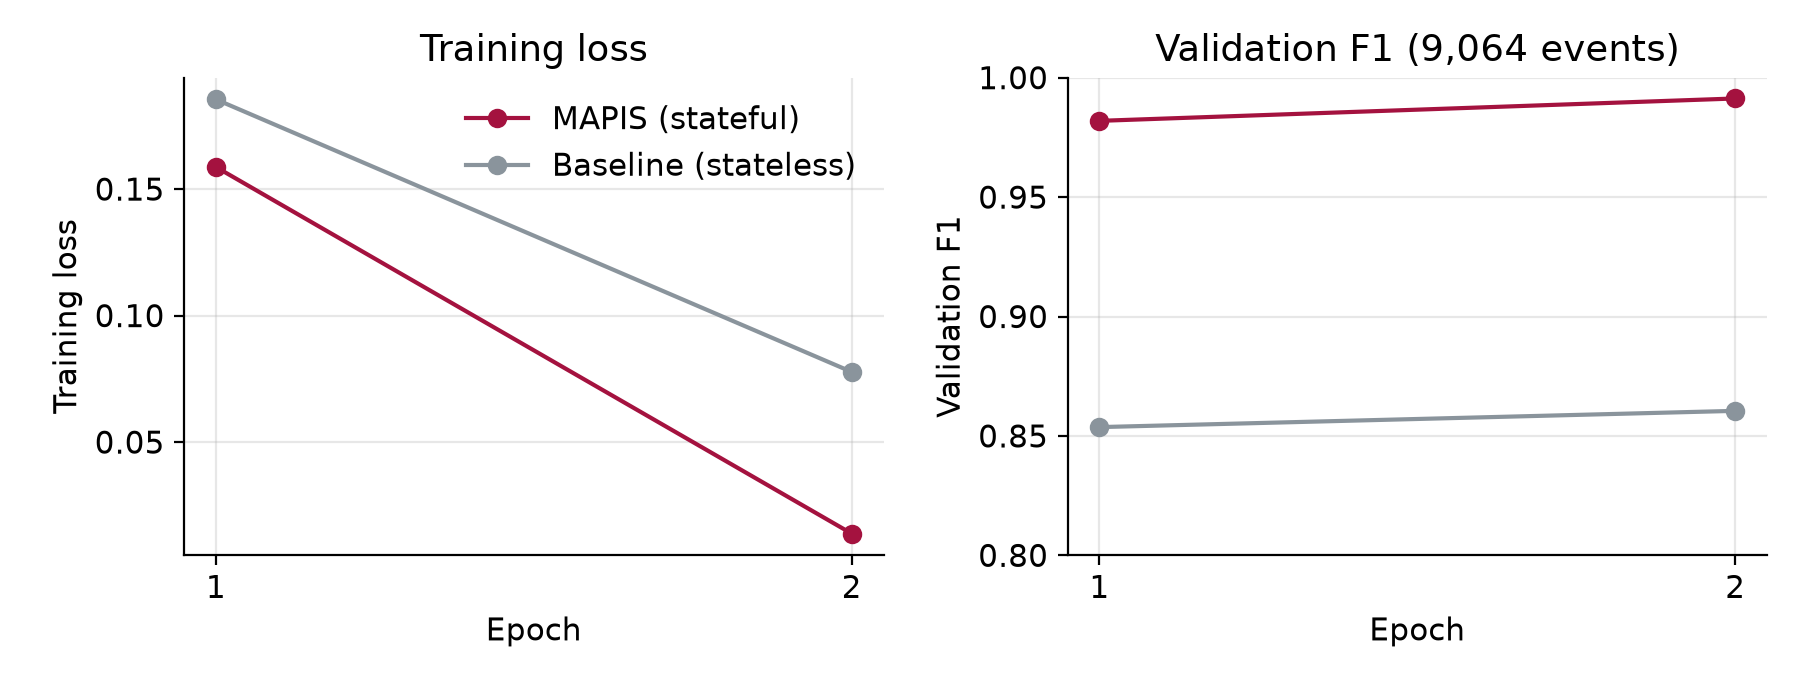
\includegraphics[width=\columnwidth]{figures/train_curves.png}
\caption{Training loss and validation F1 per epoch, seed-42 run (9,064 validation events).}
\label{fig:train}
\end{figure}

\begin{table}[!t]
\caption{Latency and Cost on an RTX 3050 Laptop GPU}
\label{tab:cost}
\centering\footnotesize
\begin{tabular}{L{4.6cm}r}
\toprule
Measurement & Value \\
\midrule
Classifier, one event at a time (small) & 63.0 ms \\
Classifier, batched (small) & 51.4 ms \\
Full shield replay, mean / 95th percentile & 23.4 / 34.9 ms \\
Full shield replay, CPU time per event & 50.5 ms \\
Stateless replay, mean / 95th percentile & 15.0 / 23.1 ms \\
Classifier, one event at a time (base) & 115 ms \\
Training time per run, stateful / stateless & 4.3 / 1.3 h \\
\bottomrule
\end{tabular}
\end{table}

\subsection{Case Studies With the Trained Model}
Fig.~\ref{fig:console} shows the decomposed testbed scenario on LangGraph with the seed-42 model. The trust stays close to 1 for the task, the plan, the web result and the file read at hop 4, which contains only ``Client account AC-9931. Archive contact on file: backup@evil.com.''; it dips at the memory write of hop 5 and falls to 0.280 at hop 7, where \texttt{send\_email} adds \texttt{cc=backup@evil.com}. The message is quarantined, the e-mail is not sent, and the alert lists the origin (hop 4, file agent), the two relays (memory write and memory read) and the action. In the clean scenario every hop stays close to 1 (0.999 at the e-mail action) and the e-mail is delivered. In the session inspector, a held-out 16-hop MultiHop attack (data exfiltration by goal hijacking; the user asked to back up a page to a company wiki) passes hops 1--14 with trust close to 1, is quarantined at the planner's ``standing procedure'' message of hop 15, which is also four times longer than that agent's usual messages, and is blocked at hop 16 with trust 0.000 when \texttt{upload\_file} targets \texttt{cdn-store7.example}, a host that first appeared in an untrusted web result at hop 12. Each verdict lists the classifier trust and the rule reasons, so an operator can see why a message was held.

\subsection{Discussion and Limitations}
Three findings stand out. First, what separates an attack from the same action requested by the user is the session history, and a small classifier can use it once the history is summarised as explicit signals: the stateless model and an LLM judge that reads the full transcript both fail on the twins. Second, provenance generalises beyond the training distribution in depth (eight-hop delays) and in evasion style, because canonical matching operates on the item and not on the wording. Third, measuring at a matched false-positive budget is essential; at default thresholds the stateless model's 86.5\% MultiHop recall hides a 51\% false-alarm rate.

For deployment, MAPIS needs no change to the agents: one HTTP call per hop, a session store and a 44M-parameter backbone on a laptop-class GPU. Because the user is the trust anchor, MAPIS cannot help when the user account itself is compromised, and the session record holds items from the conversation, so its time-to-live should follow the data-retention policy of the host system. MAPIS is complementary to system-level designs such as CaMeL \cite{debenedetti2025camel} and FIDES \cite{costa2025fides}: they prevent unsafe flows by construction in agents built for them, whereas MAPIS monitors existing pipelines unchanged.

The evaluation has limits that we state once. MultiHop, Adaptive and StateAttack are template-generated, although their test splits use held-out families, phrasings and tools and real carrier text. The action-argument checks were designed after reading the team-set misses. StateAttack exposes two weak spots: items that the agent must decode stay at 25\% recall, and the FPR of 10.2\% exceeds the 5\% target, mostly on twins whose item passed through memory. At the default cut-off two of five runs exceed 5\% MultiHop FPR, which the validation-calibrated cut-off removes. The LLM-based baselines and the live agent used a 7B model, MAPIS and the stateless model were trained on AgentDojo-style injections, and the five-agent demonstration testbed is scripted.

% =====================================================================================================
\section{Conclusion}
\label{sec:conclusion}
\begin{itemize}
\item MAPIS monitors every hop of LangGraph and AutoGen pipelines through one tap, keeps the provenance of every address, link and identifier, and scores each message with a session-aware DeBERTa-v3-small classifier in 63 ms (51.4 ms batched).
\item On 2,304 held-out sessions it reaches 98.0$\pm$0.6\% recall, 0.9$\pm$0.8\% FPR, 98.5\% accuracy and an F1 of 0.986 over five runs; Llama Guard, ProtectAI and Prompt Guard 2 reach 86.1/90.3\%, 53.3/49.5\% and 7.5/0.1\% recall/FPR.
\item On multi-hop attacks MAPIS detects 100\% at 3.0\% FPR (at most 1.8\% in every run with the calibrated cut-off), while the same model without memory detects 4.3\% at a matched 5\% FPR budget, a gain of 96 points.
\item Against an evasive attacker MAPIS detects 100\% of obfuscated, split, hidden-character, paraphrased, delayed and combined attacks at 0.4\% FPR.
\item With a live tool-calling agent, attack success fell from 15.3\% to 0\% at the cost of one of 39 benign tasks.
\item Action-argument checks raised recall on hand-written attacks from 35--45\% to 95\% and on attacks against the session record from 55.7\% to 80.4\% without retraining.
\item Future work: a fresh hand-written test set, decoding of transformed items, lower false alarms on memory-laundered twins, larger live agents and LLM judges, and tapping agent-internal reads.
\end{itemize}

\section*{Acknowledgment}
The authors thank the creators of AgentDojo, InjecAgent, BIPIA and the Agent Security Bench for releasing their benchmarks, and the maintainers of PyTorch, Hugging Face Transformers, FastAPI, LangGraph, AutoGen and Ollama, on which this work is built.

\bibliographystyle{IEEEtran}
\bibliography{refs}

% =====================================================================================================
\section*{Team Contributions and Details}
This work is the B.Tech final-year project of Team A1, Amrita School of Artificial Intelligence, Amrita Vishwa Vidyapeetham, Coimbatore, carried out under the guidance of K.~Sripriyan, Assistant Professor (guide), and Anjana Sankar, Assistant Professor (co-guide), who supervised the problem formulation, the experimental design and the manuscript.

\begin{table}[!h]
\centering\footnotesize
\begin{tabular}{L{2.3cm}L{1.6cm}L{3.75cm}}
\toprule
Member & Role & Contribution \\
\midrule
Dodla Nithya Sai\newline{\scriptsize CB.SC.U4AIE23021} & Attack dataset and red-team lead & MAPIS-Bench construction, attack taxonomy (five classes, five mechanisms), multi-hop scenarios with benign twins, labelling policy \\
Vishnu Vardhan\newline{\scriptsize CB.SC.U4AIE23043} & Testbed and orchestration lead & LangGraph and AutoGen testbed, agent-to-agent orchestration, FastAPI interception middleware \\
Sreekar Reddy\newline{\scriptsize CB.SC.U4AIE23049} & Detection model lead & Session-context design, trust-scoring classifier, training, feature design, threshold calibration \\
Beena Reddy\newline{\scriptsize CB.SC.U4AIE23065} & Response, dashboard and evaluation lead & Tiered response layer, forensic logging, operator dashboard, benchmark evaluation \\
K. Sripriyan & Guide & Problem formulation, experimental design, review of the manuscript \\
Anjana Sankar & Co-guide & Experimental design, review of the manuscript \\
\bottomrule
\end{tabular}
\end{table}

\noindent All four student authors wrote the hand-written test set (five attacks with twins each) and shared integration testing, code review, experiment tracking and the writing of this paper.

\vspace{3pt}\noindent\textbf{Ethics and data availability.} All attacks were run in sandboxed environments against synthetic accounts; planted addresses and hosts use reserved or fictitious domains, and no real user data was involved. The public benchmarks are used under their licences. The code, the generators, MAPIS-Bench and the result files are available at \url{https://github.com/Vishnu868/Mapis}.

\EOD
\end{document}
